\newpage
\section{Data Warehouse mit NoSQL[AA]}
\subsection{Load in Python}
\subsubsection{Redis Client}
\begin{figure}[H]
\centering
  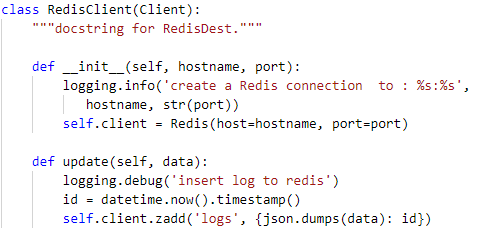
\includegraphics[scale=0.8]{images/RedisClient.PNG}
  \caption[Redis Client]{Redis Client}
  \label{fig:Redis-Client}
\end{figure}
In dem folgenden Code Block \ref{fig:Redis-Client} wird der Load Connector für Redis gezeigt. Es gibt zwei Funktionen dieser Klasse. Einerseits die Init Methode \ref{ssec:Init-Redis}, andererseits die Update Methode. \ref{ssec:Update-Redis}\\
\paragraph{Init}\mbox{}\label{ssec:Init-Redis} \\
Durch das Redis Modul in Python kann ein Client mit der Redis Datenbank einfach verbunden werden. Die einzigen Werte die die In Memory Datenbank Methode benötigt ist der Host und der dazugehörigen Port. Der Host ist die IP Adresse der Redis Datenbank und der Port lässt die Verbindung zwischen Client und 
Datenbank zu.\\
\paragraph{Update}\label{ssec:Update-Redis}\mbox{} \\
Bei der Update Methode wird klar, dass nicht eine Standard Redis Datenbank verwendet wird, sondern eine die Json Dateien entgegennehmen kann. Dies ist das Rejson Plugin \ref{ssec:Rejson}. Mit dem Client kann so ein ganzes Json File entgegengenommen und diese in die Redis Datenbank gespeichert werden. Die Id ist ein Zeitstempel um zu hinterlegen, wann die Daten in Redis gespeichert wurden.  
\newpage
\subsubsection{Rejson}\label{ssec:Rejson}
Für diesen Abschnitt sind folgende Informationen verarbeitet worden. (vgl. \cite{redislabs_rejson_2020})
\paragraph{Allgemein}\mbox{} \\
Dieses Plugin von Redis ermöglicht es mit Json Dateien in Redis zu arbeiten. Es gibt hier zwei neue Funktionen. Diese wären JSON.SET \ref{ssec:JSONSET} und JSON.GET. \ref{ssec:JSONGET}
\paragraph{JSON.SET}\mbox{}\label{ssec:JSONSET} \\
Diese Funktion erkennt die Schlüssel- und Werteaufteilung, getrennt durch einen Doppelpunkt. So wird der Wert links vom Doppelpunkt als Schlüssel hergezogen während rechts der Wert für den dazugehörigen Schlüssel steht.
\begin{figure}[H]
\centering
  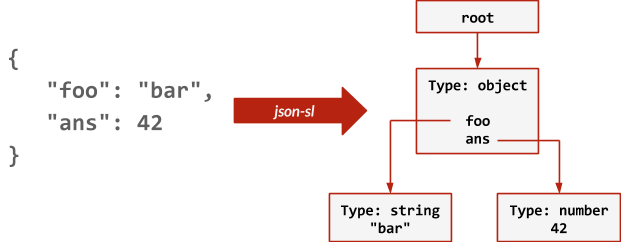
\includegraphics[scale=0.5]{images/rejson_tree.png}
  \caption[Rejson Tree (01.04.2020)]{Rejson Tree (01.04.2020)}
  \url{https://redislabs.com/wp-content/uploads/2017/03/rejson_tree.png}
  \label{fig:Rejson-Tree}
\end{figure}
Diese Graphik \ref{fig:Rejson-Tree} zeigt wie die einzelnen Objekte des Json Objekts aufgeteilt werden und den dazugehörigen Datentyp des Wertes zugeteilt bekommen. 
\paragraph{JSON.GET}\mbox{}\label{ssec:JSONGET} \\
Ganz anders wird der Schlüssel bei JSON.GET angegeben um den dazugehörigen Wert zu bekommen.
\subsubsection{Cassandra Client}
\begin{figure}[H]
\centering
  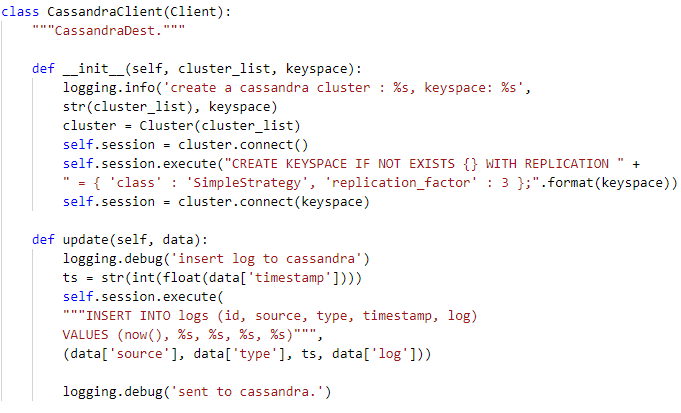
\includegraphics[scale=0.65]{images/CassandraClient.PNG}
  \caption[Cassandra Client]{Cassandra Client}
  \label{fig:Cassandra-Client}
\end{figure}
Wie zuvor ist der Code Block für den Cassandra Client \ref{fig:Cassandra-Client} gleich aufgebaut wie  für Redis \ref{fig:Redis-Client}. Auch hier gibt es die Init \ref{ssec:Init-Cassandra} und Update Funktion \ref{ssec:Update-Cassandra}.
\paragraph{Init}\mbox{}\label{ssec:Init-Cassandra} \\
Die Init Funktion bezieht sich auf das Modul von Cassandra.Cluster. In der Cluster List stehen die einzelnen Ip Adressen der Cluster mit denen sich der Client verbinden soll. Falls ein spezieller Port benutzt wird, kann der Port auch mitgegeben werden um sich zu jeden Cluster verbinden zu können. Danach wird die Verbindung zu den verschiedenen Clustern aufgebaut und in die Session gespeichert. Nach diesem Schritt wird falls der Keyspace noch nicht existiert, wird dieser dann erstellt. Ein Keyspace wäre eine eigene Unterdatenbank, wenn es gleichgesetzt werden müsste mit einer relationale Datenbanken. Als letzten Schritt der Init Funktion wird sich erneut mit dem Cluster verbunden, jedoch wird nun der Keyspace mitgegeben um so nur auf diesem zu arbeiten.\\
\paragraph{Update}\label{ssec:Update-Cassandra}\mbox{} \\
Wie zuvor bei der Init Funktion wird die Session verwendet um einen Insert durchführen zu können. Zuvor bekommt diese Funktion die Daten, als Json Format die eingefügt werden sollen. Mit diesem Insert werden die folgenden Daten in die Tabelle Cust Import eingefügt. Nach diesem Aufruf zur Cassandra Datenbank ist die Update Funktion vollendet. 
\subsubsection{Main Load}
\begin{figure}[H]
\centering
  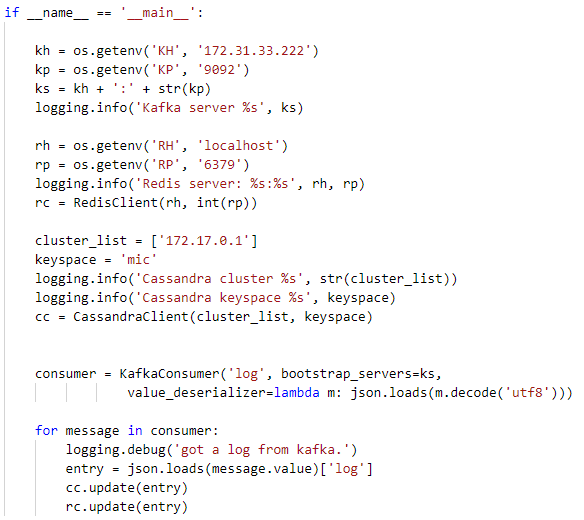
\includegraphics[scale=0.6]{images/MainLoad.PNG}
  \caption[Load]{Load}
  \label{fig:Load}
\end{figure}
\paragraph{Kafka Server}\mbox{} \\
Die ersten drei Zeilen der Main Methode fügen die Ip Adresse mit dem dazugehörigen Port zusammen. Dieser zusammengefügte String wird später verwendet um auf das Topic von Kafka zuzugreifen und von dort die Daten zu bekommen. 
\paragraph{Redis Client}\mbox{} \\
Wie zuvor werden in diesen Code Zeilen die Ip Adresse und Port angelegt und weiter an die Redis Client Klasse\ref{fig:Redis-Client} geschickt. 
\paragraph{Cassandra Client}\mbox{} \\
Anders als zuvor wird die Cluster List und der Keyspace als einfache Strings angelegt und gleich an den Cassandra Client\ref{fig:Cassandra-Client} weitergeleitet. 
\paragraph{Consumer}\mbox{} \\
Der Kafka Consumer benutzt den zuvor zusammengesetzten Kafka Ip Adressen String und bekommt das Topic zu den sich der Consumer anmelden muss mitgegeben. 
\paragraph{Message in die Datenbanken}\mbox{} \\
Nach dem alle Nachrichten in den Consumer geladen worden sind, wird jede einzelne Nachricht durchgegeben und zu einem Json Objekt übersetzt. Danach werden die Nachrichten an die Update Methode von Cassandra \ref{ssec:Update-Cassandra} und Redis \ref{ssec:Update-Redis} weitergeleitet.
\subsection{Cassandra als Data Warehouse}
\subsubsection{Allgemein}
Cassandra eignet sich gut als Raw Data Storage oder als finales Data Warehouse. Die Form der Wide Column Datenbank erinnert an eine relationale Datenbank. Zusätzlich ist es möglich die Schemata vom Data Warehouse umzusetzten. Doch ist es auch möglich durch Json verschachtelte Objekte Data Warehouse Modelle umzusetzten. Außerdem ist Cassandra eine NoSQL Datenbank die sich auf Avalability und Partitioning stützt und dazu, weil es eine NoSQL Datenbank ist um einiges schneller agieren kann als eine relationale Datenbank. Bei einem Data Warehouse ist es nicht wichtig, dass das Core Data Warehouse immer Konsistent ist. Wegen diesen Gründen ist es eine gute Idee Cassandra als Core Data Warehouse beziehungsweise als Data Mart zu benützen.
\subsubsection{Datenstruktur}
\begin{figure}[H]
\centering
  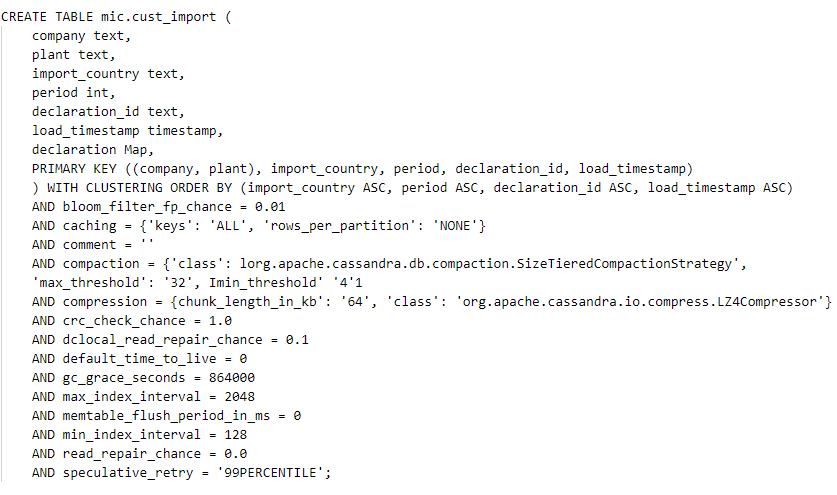
\includegraphics[scale=0.5]{images/Cassandra_Create_Table.PNG}
  \caption[Create Table]{Create Table}
  \label{fig:Create-Table}
\end{figure}
Die einzelnen Werte bedeuten folgendes:
\begin{itemize}
\item{Company}\mbox{}\\
In diesem Wert steht der Name des Unternehmens drinnen von denen die Daten vorhanden sind. Es ist möglich mehrere Daten des gleichen Unternehmens zu haben. 
\item{Plant}\mbox{}\\
Hier werden die Werke des Unternehmens gespeichert.
\item{Import Country}\mbox{}\\
Zur Analyse ist es wichtig das Land mit abzuspeichern von welche die Import stammen. 
\item{Period}\mbox{}\\
Eines der wichtigsten Werte in der Tabelle ist die Periode um Analysen durchführen zu können. 
\item{Load Timestamp}\mbox{}\\
Dieser Wert ist dazu da um abzuspeichern, wann ein neuer Eintrag in die Tabelle eingetragen wird.
\item{Declaration Id}\mbox{}\\
Diese Id ist wichtig wenn die Declaration eingebunden werden soll.
\item{Declaration}\mbox{}\\
Der letzte Wert ist eine Zusammenfassung aller Dimensionstabellen wäre es ein relationales Data Warehouse. Dazu ist der Map Datentyp dazu da um eine eigene Kollektion von Schlüssel Werte Paare zu sichern. Dadurch ist es möglich so ein Data Warehouse in einer einzelnen Tabelle zu halten. Durch die Eigenschaften von NoSQL kann auf diesen Datentyp schnell zugegriffen werden. 
\end{itemize}
\newpage
\subsection{Rest Server}
\subsubsection{Get Uids}
\begin{figure}[H]
\centering  
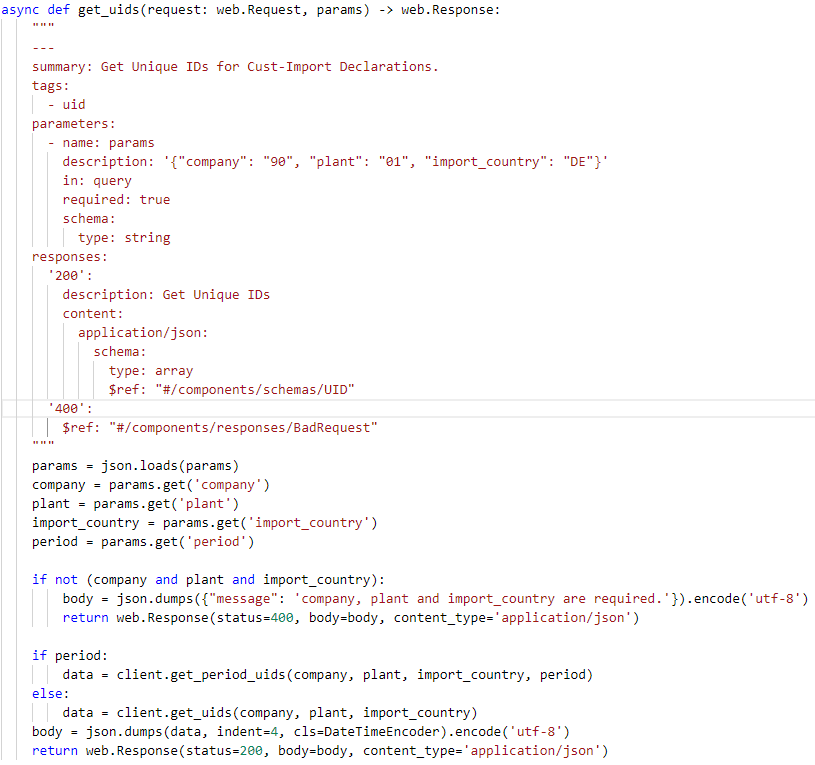
\includegraphics[scale=0.55]{images/GetUids.PNG}
  \caption[Get Uids]{Get Uids}
  \label{fig:Get-Uids}
\end{figure}
Diese Methode gibt alle UIDs durch einen Rest Aufruf zurück. Am Anfang werden die Parameter auf ein Json Format konvertiert. Nach dieser Umstellung auf Json werden alle relevanten Daten, das Unternehmen, das Werk, das Land und die Periode in eigene Variablen abgespeichert.\\


Falls das Unternehmen, das Werk oder das Land fehlt wird ein Bad Request zurückgegeben und es wird aufgefordert alle relevanten Daten anzugeben.\\

Wenn alles in Ordnung ist gibt es zwei unterschiedliche Wege wie die UIDs zurückgegeben werden. So können, wenn die Periode angegeben wird nur die Daten in dieser gewissen Zeit zurückgegeben werden. Andererseits, wenn die Periode nicht angeben wird, werden alle Daten des Unternehmens mit diesem Werk in diesem Land zurückgegeben.
\subsubsection{Get Declaracions}
\begin{figure}[H]
\centering
  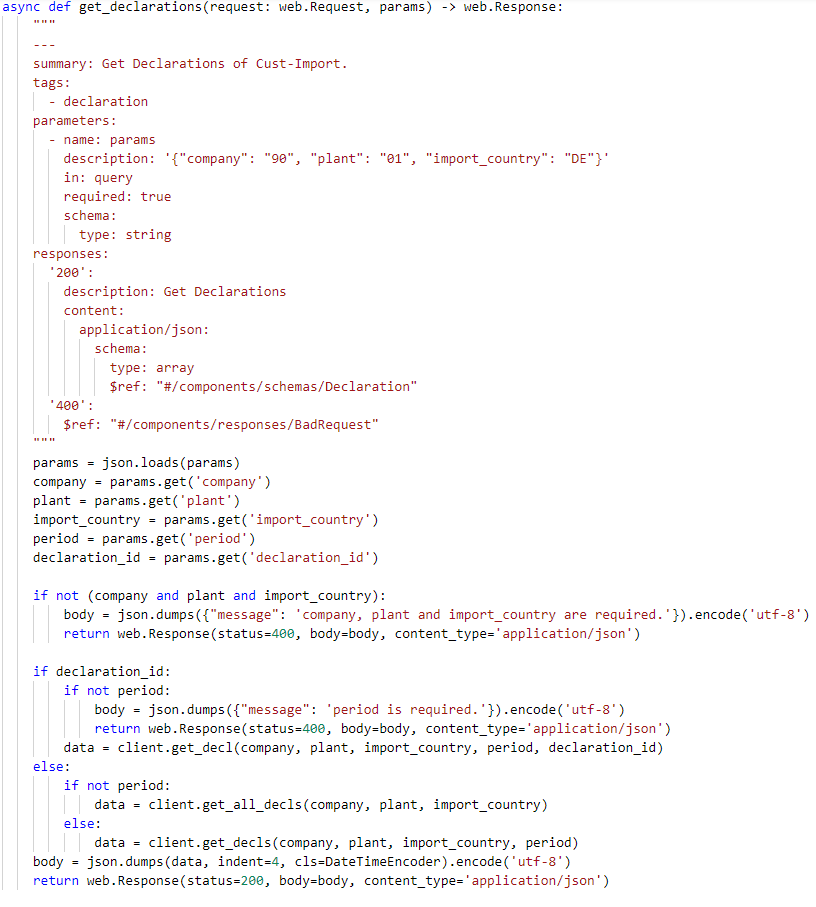
\includegraphics[scale=0.5]{images/GetDeclaracions.PNG}
  \caption[Get Declaracions]{Get Declaracions}
  \label{fig:Get-Declaracions}
\end{figure}
Wie zuvor auch werden als erstes die Parameter auf ein Json Objekt umgemappt um so abgespeichert werden zu können.\\

Auch in diesem Aufruf ist es notwendig das Unternehmen, das Werk und das zugehörige Land anzugeben. Der Unterschied liegt darin, dass nun zusätzlichen zu diesen Werten die Declaration Id hinzugefügt werden kann. Falls diese angegeben wird ist es auch nötig die Periode die beobachtet werden soll mitzugeben. Falls dies nicht der Fall ist wird ein Bad Request abgegeben der auffordert eine Periode anzugeben.\\

Genau wie zuvor werden sonst die ausgewerteten Daten mitgegeben und weiter an den Visualisierungsprozess geschickt. Entweder von einer bestimmten Deklaration also ein bestimmtes Produkt oder alle Deklarationen eines Unternehmens.
\subsubsection{Main Rest}
\begin{figure}[H]
\centering
  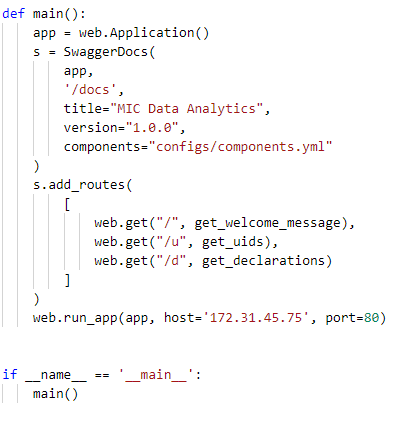
\includegraphics[scale=0.6]{images/MainRest.PNG}
  \caption[Rest]{Rest}
  \label{fig:Rest}
\end{figure}
In der Main Methode des Rest Servers wird als erstes der Wert der Web Applikation in eine eigene Variable gelegt. Danach wird ein SwaggerDoc \ref{ssec:SwaggerDoc} erstellt um die Rest Aufrufe besser bedienen und aufrufen zu können. In diesem SwaggerDoc wird die Applikation selbst sowie Aufrufpfad, Titel, Version und Komponenten hinzugefügt.\\

Nach dem dieses Swaggerdoc erstellt und gespeichert wurde, werden nun die einzelnen Routen zu den Rest Aufrufen hinterlegt. So leitet nun /u zu der Get UIDs Methode \ref{fig:Get-Uids} während /d auf Get Declarations \ref{fig:Get-Declaracions} verweist.\\

Am Ende wird der Rest Server selbst ausgeführt und kann auf Port 80 mit der Ip Adresse 172.17.0.1 angesprochen werden.
\subsubsection{AioHttp}
AioHttp ist ein Paket, dass Server und Client unterstützt. Durch dieses Modul ist es einfach einen Rest Server mit Python zu realisieren und wenn es nötig ist leicht Websocket Verbindungen zu verwalten. Ein großer Vorteil von AioHttp ist es, dass die Routen zu den Aufrufen leicht zu realisieren und zu überprüfen sind. 
\subsubsection{SwaggerDocs / AioHttp-Swagger3}\label{ssec:SwaggerDoc}
Dieses Modul wird dazu verwendet um Rest Aufrufe durch Header Kommentare umzusetzten. Wie in der Abbildung \ref{fig:Get-Uids} \& \ref{fig:Get-Declaracions} kann so ein viel schönerer und klarerer Überblick über die Funktion eines Rest Aufrufs getätigt werden. Der Name stammt daher das es die Spezifikationen von Swagger 3.0 übernimmt. Das Modul heißt auch OpenAPI3. 
